% Created 2020-06-29 Mon 09:54
% Intended LaTeX compiler: pdflatex
\documentclass[presentation]{beamer}
\usepackage[utf8]{inputenc}
\usepackage[T1]{fontenc}
\usepackage{graphicx}
\usepackage{grffile}
\usepackage{longtable}
\usepackage{wrapfig}
\usepackage{rotating}
\usepackage[normalem]{ulem}
\usepackage{amsmath}
\usepackage{textcomp}
\usepackage{amssymb}
\usepackage{capt-of}
\usepackage{hyperref}
\usetheme{UoB}
\author{Mark Blyth}
\date{\textit{[2020-06-30 Tue]}}
\title{More model fitting}
\hypersetup{
 pdfauthor={Mark Blyth},
 pdftitle={More model fitting},
 pdfkeywords={},
 pdfsubject={},
 pdfcreator={Emacs 26.3 (Org mode 9.1.9)}, 
 pdflang={English}}
\begin{document}

\maketitle

\section{Intro}
\label{sec:orgcc7a41d}
\begin{frame}[label={sec:org75258e4}]{Presentation points}
\begin{itemize}
\item Models for wind tunnel data
\item A BARS redesign
\item BARS potential pitfalls
\end{itemize}
\end{frame}

\begin{frame}[label={sec:org9d899c8}]{An exciting aside}
\begin{center}
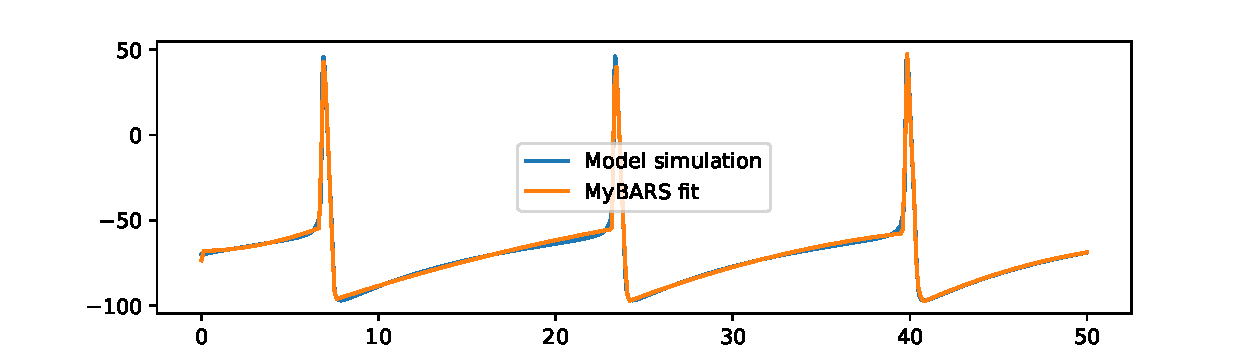
\includegraphics[width=.9\linewidth]{./mybars.pdf}
\end{center}

My BARS implementation works! 
\begin{itemize}
\item Gives okay results \emph{[some sharp corners?]}
\item Allows arbitrary interpolation
\item Slower than the C implementation
\end{itemize}
\end{frame}

\section{Wind tunnels}
\label{sec:orgf968e6b}
\begin{frame}[label={sec:org1799d62}]{BARS - wind tunnel}
\begin{center}
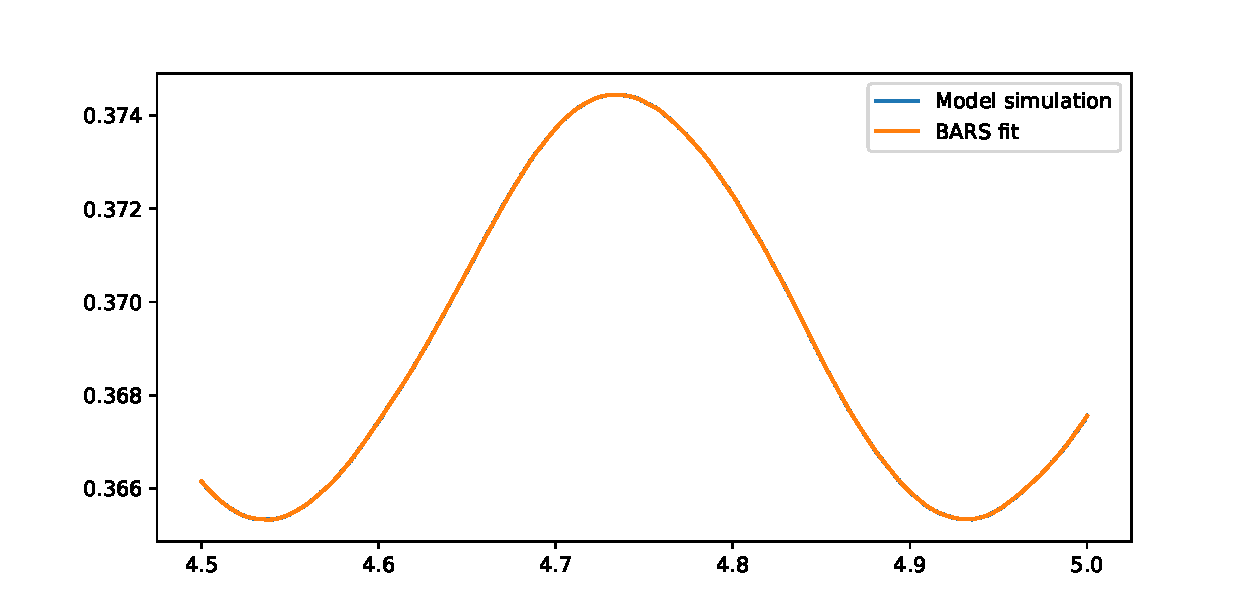
\includegraphics[width=.9\linewidth]{./bars_section.pdf}
\end{center}

2500 datapoints, 41s run-time
\end{frame}

\begin{frame}[label={sec:org6e62813}]{BARS - wind tunnel}
\begin{center}
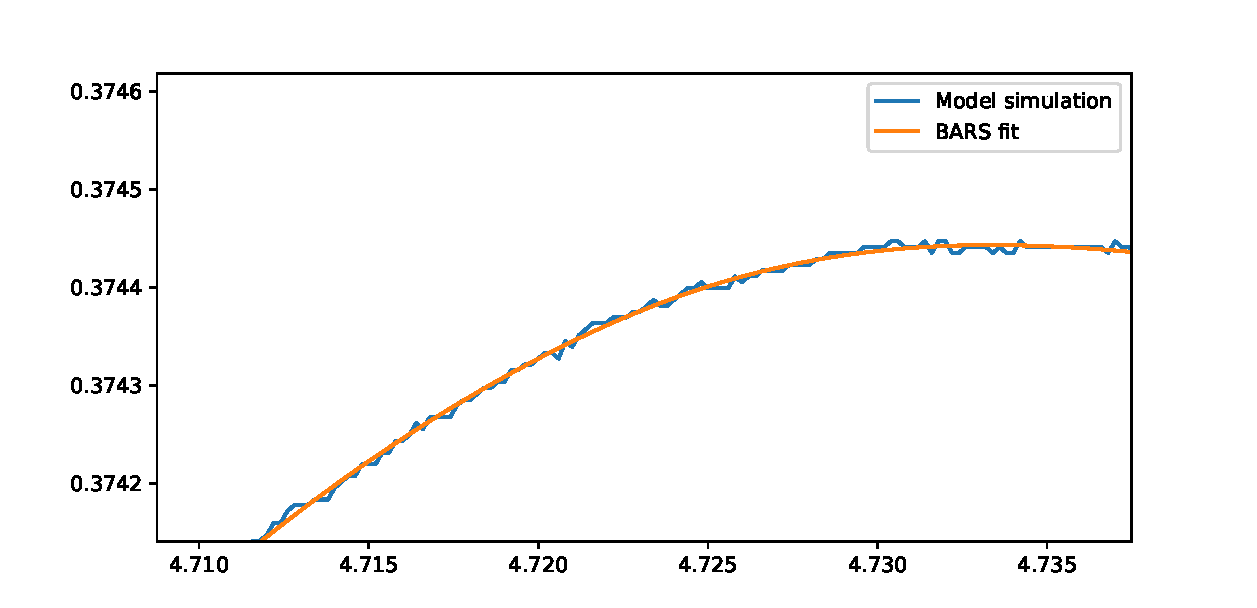
\includegraphics[width=.9\linewidth]{./bars_zoom.pdf}
\end{center}

2500 datapoints, 40s run-time
\end{frame}

\begin{frame}[label={sec:orge4b0e07}]{Matern32 (GPR) - wind tunnel}
\begin{center}
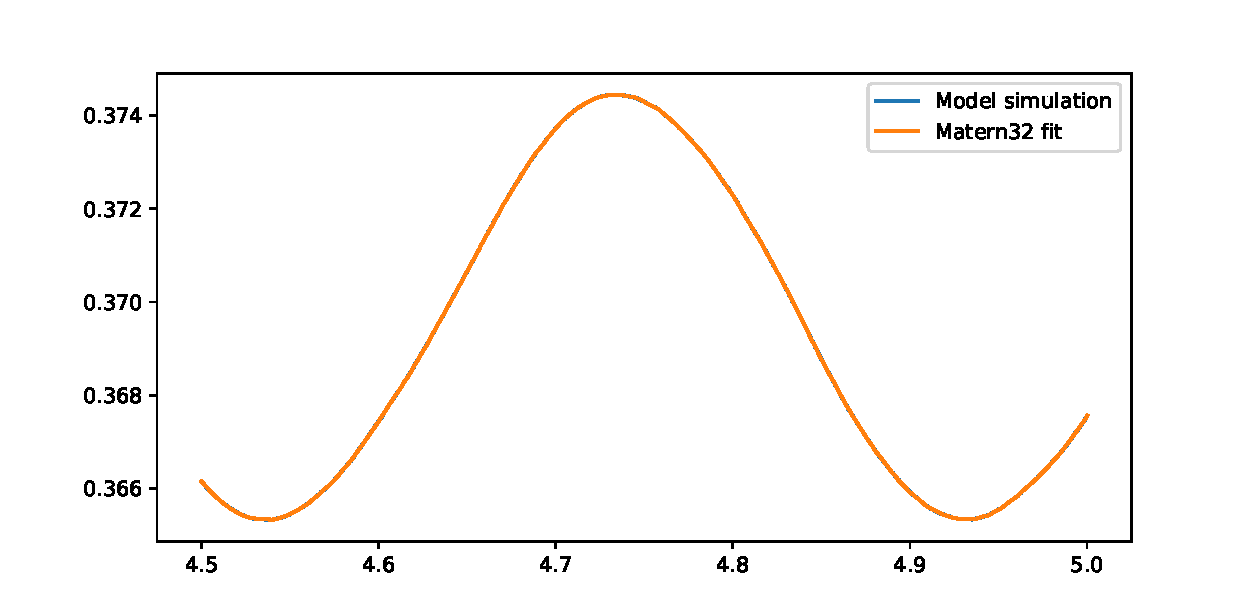
\includegraphics[width=.9\linewidth]{./matern32section.pdf}
\end{center}

2500 datapoints, 119s run-time
\end{frame}

\begin{frame}[label={sec:org624ca13}]{Matern32 (GPR) - wind tunnel}
\begin{center}
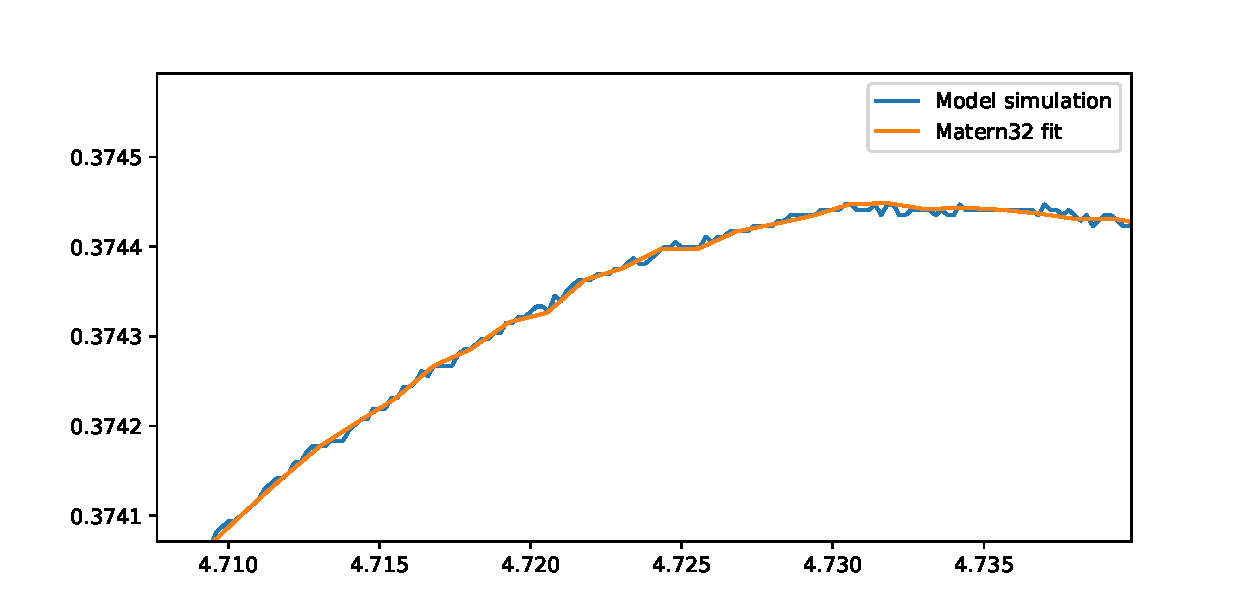
\includegraphics[width=.9\linewidth]{./matern32zoom.pdf}
\end{center}

2500 datapoints, 119s run-time
\end{frame}

\section{Issues}
\label{sec:orgc897808}
\begin{frame}[label={sec:orgc3f11b1}]{Timings}
\begin{itemize}
\item Unoptimized C code is still faster than optimized python / matlab
\begin{itemize}
\item BARS is using optimized C implementation, GPRs is using my unoptimized python implementation
\item GPFlow, GPyTorch would be much faster for GPR
\item Probabilistic programming might speed up BARS
\end{itemize}
\end{itemize}
\vfill
\begin{itemize}
\item Both methods are \(\mathcal{O}(n^3)\); require inverting \(n \times n\) matrix
\begin{itemize}
\item Both perform poorly on lots of datapoints!
\end{itemize}
\end{itemize}
\end{frame}

\begin{frame}[label={sec:orgcbec05c}]{BARS}
\begin{center}
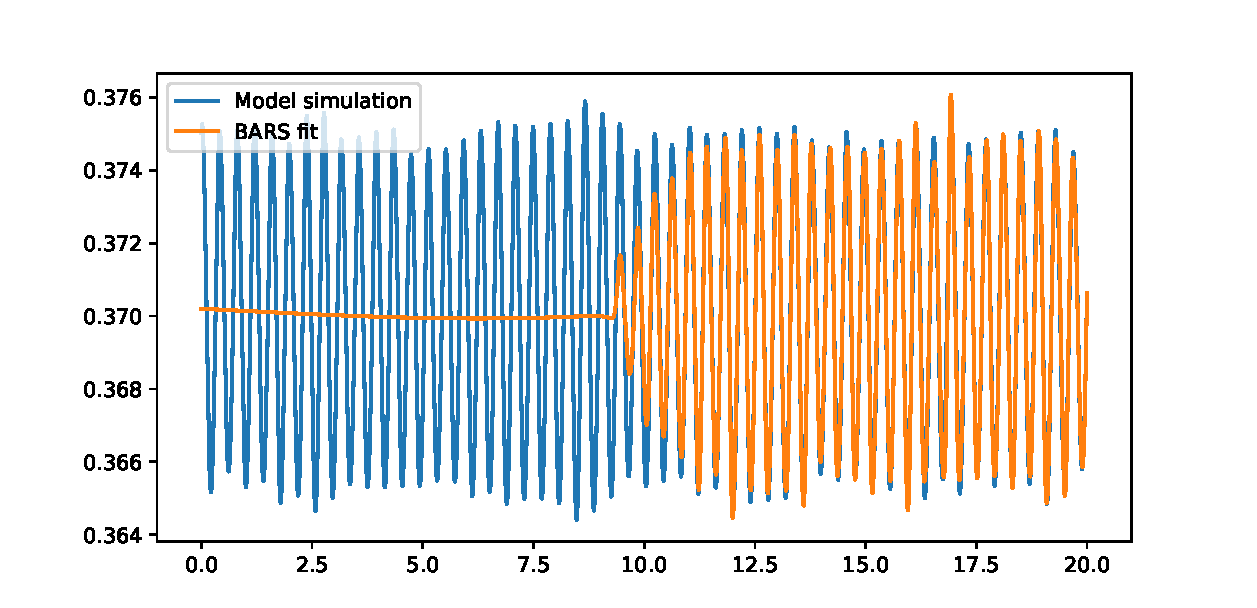
\includegraphics[width=.9\linewidth]{./barsfull1.pdf}
\end{center}

10,000 datapoints \emph{[crashes with full dataset]}, 142s run-time
\end{frame}

\begin{frame}[label={sec:org240d512}]{BARS}
\begin{center}
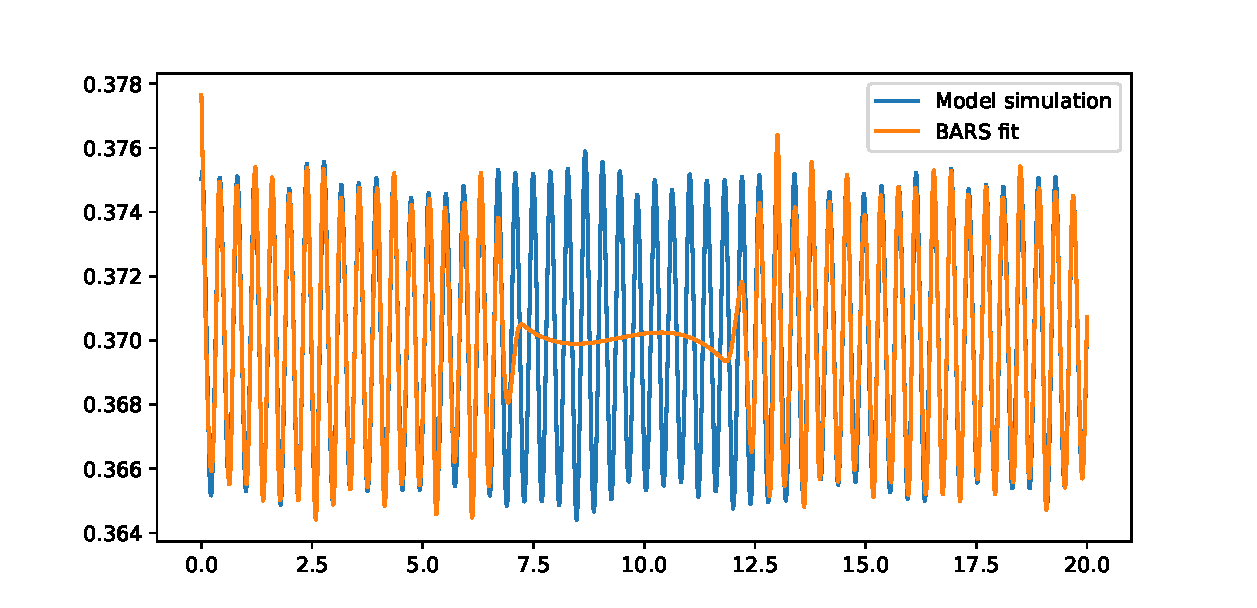
\includegraphics[width=.9\linewidth]{./barsfull2.pdf}
\end{center}

10,000 datapoints \emph{[crashes with full dataset]}, max. number of knots \emph{[80]}, more burn-in;  590s (9 mins 50s) run-time
\end{frame}

\begin{frame}[label={sec:org50e32b7}]{BARS issues}
\begin{itemize}
\item C implementation doesn't allow validation
\begin{itemize}
\item Can't interpolate at arbitrary points
\item Python implementation does! But it's slower
\end{itemize}
\item C implementation caps the max. number of knots
\begin{itemize}
\item Python implementation doesn't! But it's slower
\item Doesn't work for long time series
\end{itemize}
\item \(\mathcal{O}(n^3)\) means data need downsampling to be used
\begin{itemize}
\item Took about 10 minutes to fit a model to 10\% of the data
\end{itemize}
\end{itemize}
\end{frame}

\begin{frame}[label={sec:orgc31c3ae}]{Experimental data}
\begin{itemize}
\item \alert{If experiments use small numbers of periods (1, 2, 3), current methods work}
\begin{itemize}
\item Similar to how I tested models on small numbers of neuron spikes
\item Few periods = less data = fewer knots needed, and quicker fit obtained
\end{itemize}
\item More datapoints mean we need to get creative\ldots{}
\begin{itemize}
\item Sparse variational BARS
\item Periodic BARS
\item Semiperiodic methods
\end{itemize}
\end{itemize}

\vfill
Or\ldots{} speed up BARS by not using BARS
\end{frame}

\section{New BARS's}
\label{sec:org65bfed9}
\begin{frame}[label={sec:orgedc71d2}]{A new BARS approach}
IDEA: Bayesian adaptive \emph{evolutionary} splines; genetic algorithm
\begin{itemize}[<+->]
\item Ideal result: find the MAP knot-config \emph{[best given data]} in fewer steps than MCMC takes to estimate posterior distribution
\begin{itemize}
\item BARS uses MCMC to find a posterior knot distribution \(p(k, \xi | y)\)
\item MCMC uses 10,000+ knot-shuffling steps to estimate this posterior distribution
\end{itemize}
\item Instead of estimating posterior distribution, why not find posterior mode?
\begin{itemize}
\item Use the knot-shuffling steps to evolve an optimal knot-set
\item Find \(\mathrm{argmax}_{k, \xi} p(y | k, \xi)\) \emph{[MLE]} \alert{\emph{or}} \(\mathrm{argmax}_{k, \xi} p( k, \xi | y)\) \emph{[MAP]}
\item Each MCMC knot-shuffle becomes a mutation step
\item Each MCMC acceptance/rejection becomes an evolutionary scoring step
\end{itemize}
\end{itemize}
\end{frame}

\begin{frame}[label={sec:orgee29cb4}]{Possible evolutionary splines implementation}
\begin{enumerate}[<+->]
\item Start with a set of initial (randomly drawn) pool of knot configurations
\item For each perturbation step\ldots{}
\begin{enumerate}
\item Randomly move, add, or delete a knot from each set
\item If the perturbed knot has a better likelihood \(p(y | k, \xi)\) than the original, replace the original with it
\end{enumerate}
\item For each epoch\ldots{}
\begin{enumerate}
\item Take \(i\) perturbation steps on each model in the pool
\item Store a pool of the \(j\) best models
\item Create a new pool by randomly recombining existing pool
\end{enumerate}
\item Pool will \emph{[hopefully]} converge to MLE
\item Can maximise posterior, instead of likelihood, by including a prior term
\end{enumerate}
\end{frame}

\begin{frame}[label={sec:org614715a}]{BARS vs evolution}
\begin{itemize}
\item Would be interesting to compare this to the MCMC method
\begin{itemize}
\item MCMC sets up a Markov chain whose stationary distribution is the posterior
\item This aims to find a Markov chain whose stationary distribution is the \(\mathrm{argmax}\)
\item Grounds for a rigorous justification / proof of convergence
\end{itemize}
\end{itemize}
\vfill
\begin{itemize}
\item Evolution will likely be faster
\begin{itemize}
\item Could leverage existing genetic optimization packages
\item Easily parallelised for more speed-up
\item No RJ-MCMC makes it easier target for probabilistic programming
\end{itemize}
\end{itemize}
\end{frame}

\begin{frame}[label={sec:org63f7bd8}]{SV-BARS}
Another idea: remodel BARS to work similarly to sparse GPR

\vfill
\begin{itemize}
\item BARS typically uses 3000+ MCMC steps
\begin{itemize}
\item Each MCMC step requires inverting an \(n \times n\) matrix -- SLOW
\end{itemize}
\item Choose a \emph{[small]} set of maximally informative surrogate datapoints \((x_i^*, y_i^*)\)
\item Run MCMC step on surrogate datapoints
\begin{itemize}
\item Much faster to invert the smaller matrix
\end{itemize}
\item Well-chosen surrogate points means we get the same result as running on real data
\item Fewer datapoints means it runs a lot faster
\end{itemize}
\end{frame}

\begin{frame}[label={sec:orgb5e7b7e}]{SV-BARS implementation}
\begin{itemize}
\item Find a set of \(m\) inducing points \((x_i^*, y_i^*)\)
\begin{itemize}
\item Find inducing points by minimising \(D_\mathrm{KL}\left[p_y \| p_{y^*}\right]\)
\item Use variational Bayes to approximate this
\end{itemize}
\item Find posterior knots \(p(k, \xi | y^*)\) \emph{[instead of \(p(k,\xi | y)\)]}
\begin{itemize}
\item \(\mathcal{O}(m^3)\), \(m\ll n\)
\item Sparse GPR is \(\mathcal{O}(nm^3)\), so if my complexity is correct, we get a bigger speed-up / outperform SVGPR!
\end{itemize}
\end{itemize}


\vfill
Would require learning RJ-MCMC, variational Bayes, sparse GPR in-depth
\end{frame}

\begin{frame}[label={sec:orgc45aa04}]{Periodic BARS}
An approach for if we need to model more than a few spikes:   
\vfill

\begin{itemize}
\item Assume data are given by \(y_i = f(x_i) + \varepsilon\)
\begin{itemize}
\item \(f(t) = f(t+T)\)
\end{itemize}
\item Find either
\begin{itemize}
\item \(T\)-periodic knot-set
\item \(T\)-periodic basis splines
\begin{itemize}
\item Nicer approach

\vfill
\end{itemize}
\end{itemize}
\end{itemize}
\ldots{}in such a way that we\ldots{}
       \vfill
\begin{itemize}
\item minimise fitting time
\item balance fit against number of knots
\end{itemize}
\end{frame}

\begin{frame}[label={sec:orgc8bc2e2}]{Semiperiodic methods}
\begin{center}
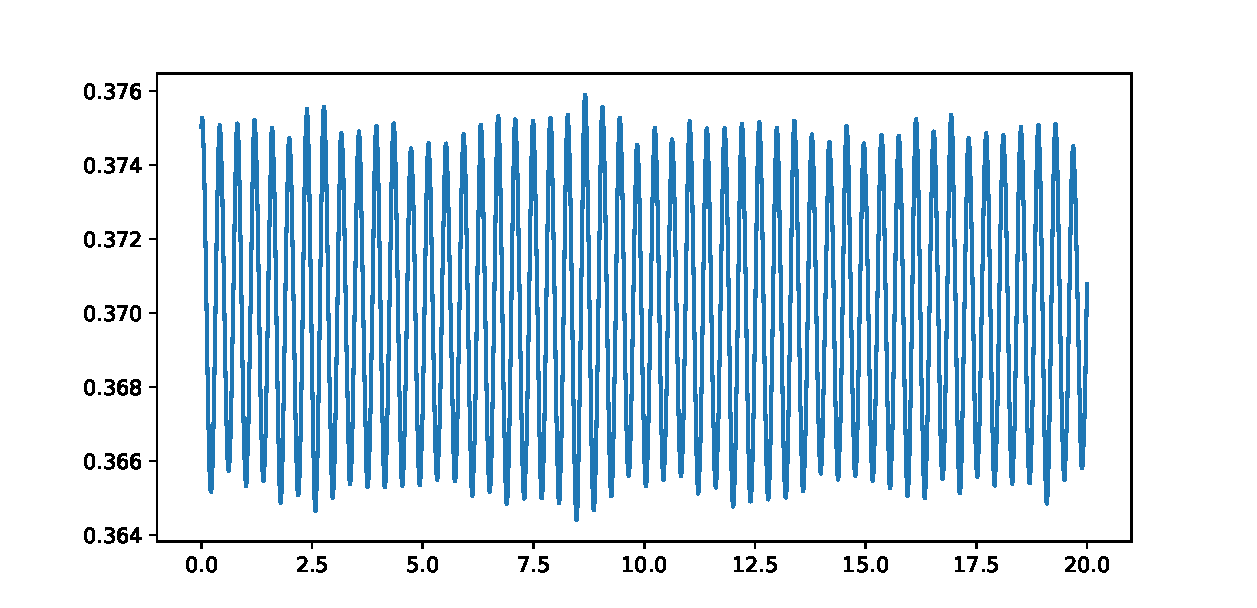
\includegraphics[width=.9\linewidth]{./nonperiodicwind.pdf}
\end{center}
Experimental data aren't perfectly periodic
\end{frame}

\begin{frame}[label={sec:orged36cfb}]{Semiperiodic methods}
\begin{center}
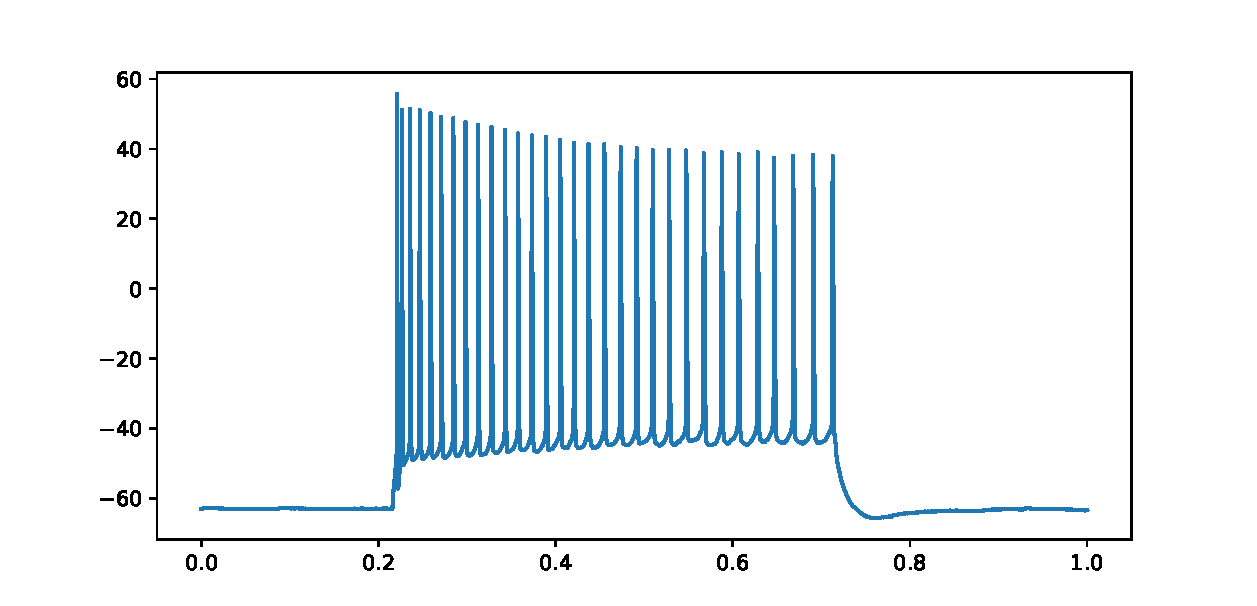
\includegraphics[width=.9\linewidth]{./mouseaperiodic.pdf}
\end{center}
Experimental data aren't perfectly periodic \emph{[could Ca\(^{\text{2+}}\), or experiment setup!]}
\end{frame}

\begin{frame}[label={sec:orgf80fb6b}]{Semiperiodic methods}
\begin{itemize}[<+->]
\item Assume data are given by \(y_i = A(x_i)f(x_i) + \varepsilon\)
\begin{itemize}
\item \(f(t) = f(t+T)\) is the periodic behaviour
\item \(A(t)\) is the drifting amplitude
\item Might require transforming the data, to a zero-DC offset
\end{itemize}
\item Fit a model to \(f(t)\)
\begin{itemize}
\item Only requires one period's worth of data
\end{itemize}
\item Fit a model to \(A(t)\)
\begin{itemize}
\item Requries a few datapoints across all periods
\end{itemize}
\item BARS, GPR, NARMAX all interesting model options
\item Would likely give similar results to sparse BARS
\end{itemize}
\end{frame}


\section{Next steps}
\label{sec:org37f59a6}
\begin{frame}[label={sec:orga9c9ba0}]{Conclusions}
\begin{itemize}[<+->]
\item For small numbers of cycles (1, 2, 3), current BARS works well enough for CBC
\item For bigger data, we need something more creative
\item Sparse variational BARS would be valuable within machine learning community
\begin{itemize}
\item Would very likely give state-of-the-art results!
\item Could be combined with the evolutionary approach for more speedup
\end{itemize}
\item (Semi)periodic BARS would be less generally applicable, but potentially faster when applicable
\end{itemize}
\end{frame}

\begin{frame}[label={sec:orgef933f5}]{Possible routes}
\begin{enumerate}[<+->]
\item Use current BARS setup for a CBC experiment
\begin{itemize}
\item Gets CBC results fast
\end{itemize}
\item Adapt current BARS setup for sparsity / evolution, then use in CBC
\begin{itemize}
\item New splines method would be valuable in ML community
\end{itemize}
\item Demonstrate splines \emph{[and GPR?]} on other problems (NDC, comp-synth-bio, ML)
\begin{itemize}
\item Extra paper, builds well on the surrogate-modelling knowledge I'm developing
\item I wouldn't know which problems to apply them to
\end{itemize}
\item Make a periodic BARS setup, then use that in CBC
\begin{itemize}
\item Periodic BARS is a less general method
\end{itemize}
\end{enumerate}
\end{frame}

\begin{frame}[label={sec:orgae3b572}]{My proposal}
\begin{itemize}
\item Validate models
\begin{itemize}
\item \alert{Also try simple data transformations for GPR}
\end{itemize}
\item Write up notes on \emph{everything} so far

\vfill
\end{itemize}
Then\ldots{}
\begin{enumerate}
\item Adapt BARS for sparsity, evolution
\begin{itemize}
\item Fast, SOTA, scalable
\item Needs variational Bayes learned
\end{itemize}
\item Demonstrate sparse BARS on other problems (NDC, comp-synth-bio, ML)
\begin{itemize}
\item Not sure which problems would benefit from splines?
\end{itemize}
\item Apply the shiny new splines method to CBC
\end{enumerate}
\end{frame}
\end{document}
